%!TEX root = report.tex
This section presents the results of the experiments with the one- and two- dimensional model discussed in \cref{s:experiment}, in \cref{ss:results:1D} and \cref{ss:results:2D}, respectively.

\subsection{One-Dimensional Model}
\label{ss:results:1D}
	\Crefrange{tab:results:1D:10:1000}{tab:results:1D:1000:10000} in \cref{a:results1D} present the results of the experiment with the one dimensional model.

	In \cref{tab:results:1D:10:1000,tab:results:1D:10:10000} we observe that the accuracy of the 1D simulation is reasonable for temperatures greater than 0.4. In the simulation with $\numberOfSpins = 10$. 
	%
	The simulation with $\numberOfSpins = 100$ starts being accurate at $\temperature = 1.4$ if $\numberOfSamples = 1000$ and at $\temperature = 0.8$ if $\numberOfSamples = 10000$. 
	%
	If we increase the number of particles to $\numberOfSpins = 1000$ we only find reasonable accuracy with $\numberOfSamples = 10000$ for $\temperature > 1.6$.

	For all values of $\numberOfSpins$ we find that the accuracy improves in general as the number of samples increases, although this effect is stronger in simulations with more spins.

\subsection{Two-Dimensional Model}
\label{ss:results:2D}
	The average energy, specific heat and average magnetization per spin for the different combinations of \numberOfSpins and \numberOfSamples can be found in \cref{fig:results:2D}. 

	\begin{figure}
		\centering
		\begin{subfigure}{\columnwidth}
			\centering
			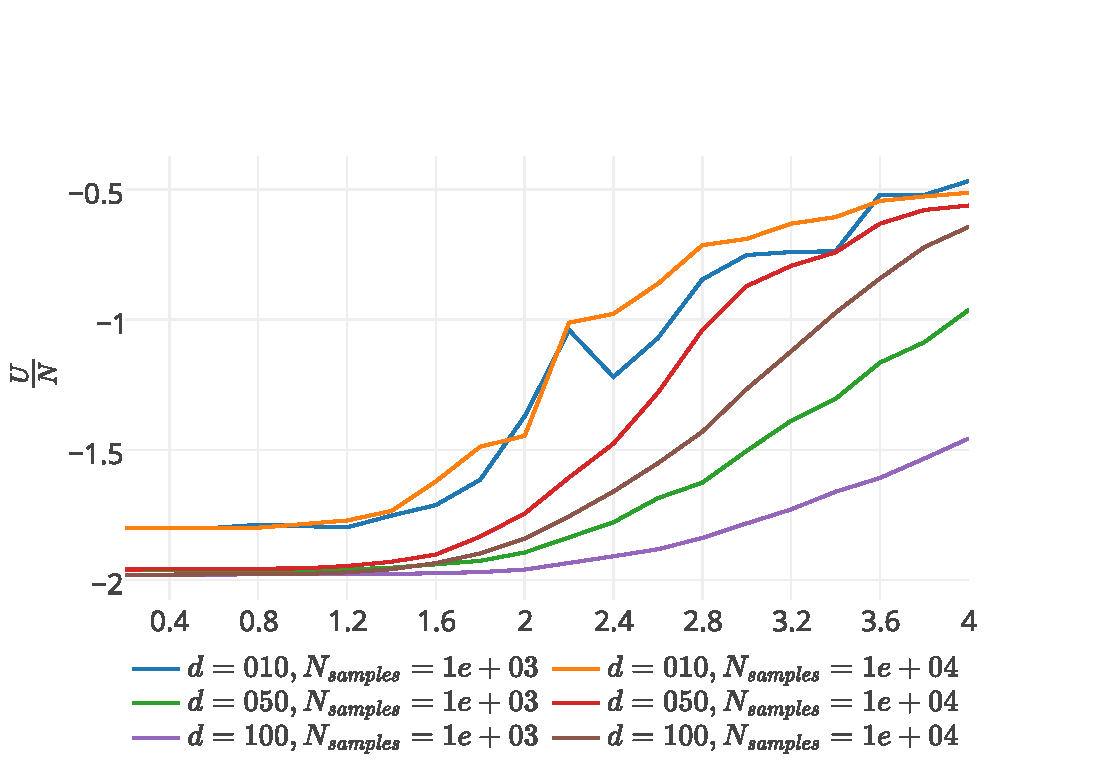
\includegraphics[width=\textwidth]{./img/2D/averageEnergy}
			\caption{Average energy per spin.}
			\label{fig:results:2D:averageEnergy}
		\end{subfigure}
		\begin{subfigure}{\columnwidth}
			\centering
			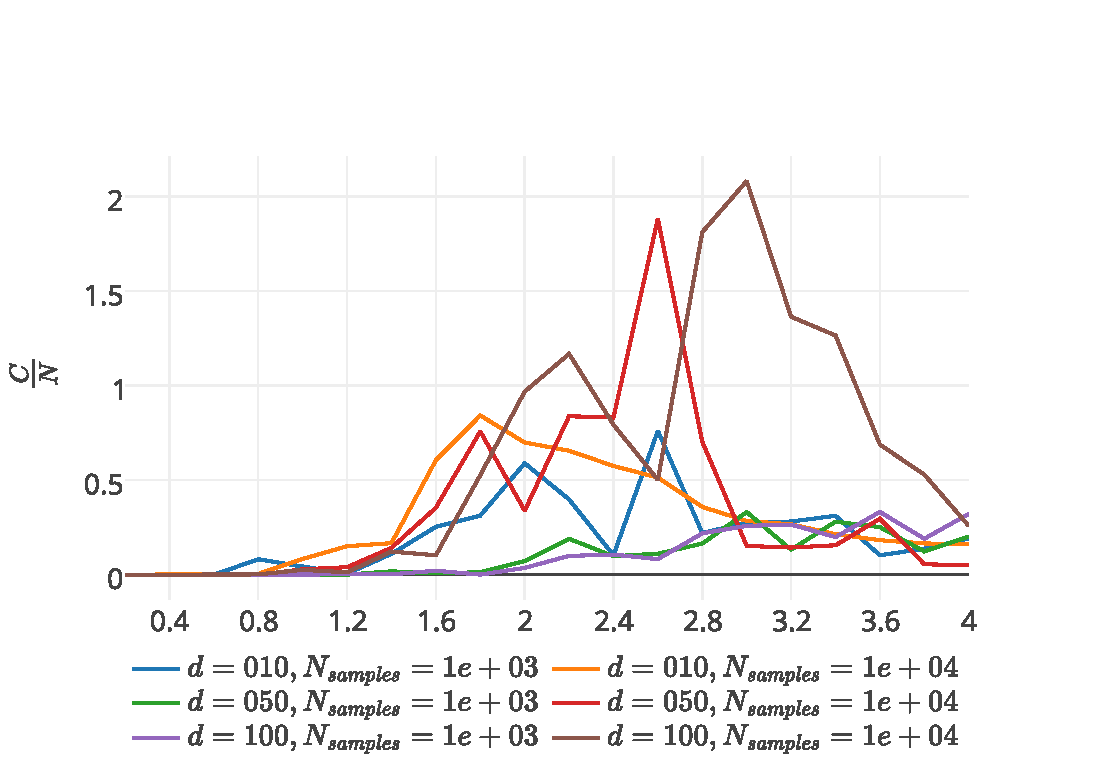
\includegraphics[width=\textwidth]{./img/2D/specificHeat}
			\caption{Average magnetization per spin.}
			\label{fig:results:2D:specificHeat}
		\end{subfigure}	
		\begin{subfigure}{\columnwidth}
			\centering
			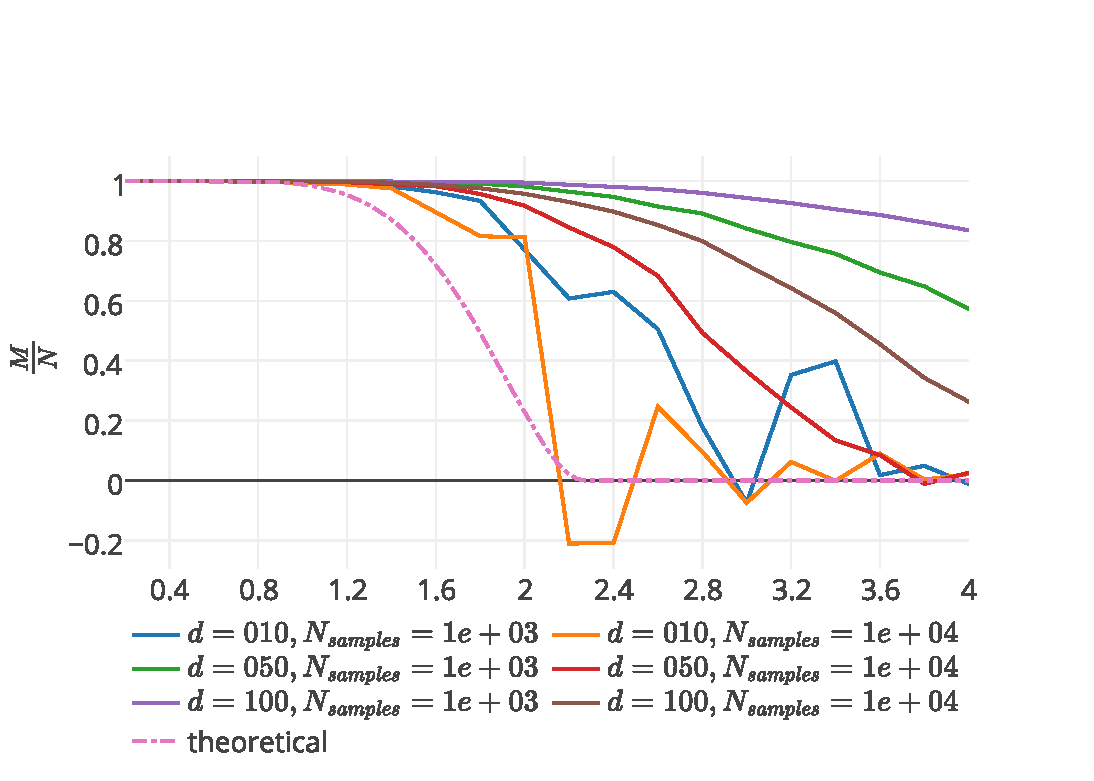
\includegraphics[width=\textwidth]{./img/2D/averageMagnetization}
			\caption{Average magnetization per spin.}
			\label{fig:results:2D:averageMagnetization}
		\end{subfigure}		
		\caption{The \subref{fig:results:2D:averageEnergy} average energy, \subref{fig:results:2D:specificHeat} specific heat and \subref{fig:results:2D:averageMagnetization} average magnetization per spin in a 2D Ising model with $\dimensionality = 10, 50, 100$ and $\numberOfSamples = 1000, 10000$.}
		\label{fig:results:2D}
	\end{figure}